% !TEX TS-program = xelatex
% !TEX encoding = UTF-8 Unicode
\documentclass[11pt,a4paper]{article}
\usepackage{amsmath,amssymb}
\usepackage{empheq}
\usepackage[semibold]{ebgaramond}
\usepackage[cmintegrals,cmbraces]{newtxmath}
\usepackage{ebgaramond-maths}
\usepackage{bm}
\usepackage[OMLmathrm, OMLmathsfit, rmdefault=mdugm]{isomath}
\usepackage{tocbibind}
\usepackage{graphicx}
\graphicspath{{./pics/}}
\usepackage{wrapfig}

\makeatletter
  \DeclareSymbolFont{ntxletters}{OML}{ntxmi}{m}{it}
  \SetSymbolFont{ntxletters}{bold}{OML}{ntxmi}{b}{it}
  \re@DeclareMathSymbol{\leftharpoonup}{\mathrel}{ntxletters}{"28}
  \re@DeclareMathSymbol{\leftharpoondown}{\mathrel}{ntxletters}{"29}
  \re@DeclareMathSymbol{\rightharpoonup}{\mathrel}{ntxletters}{"2A}
  \re@DeclareMathSymbol{\rightharpoondown}{\mathrel}{ntxletters}{"2B}
  \re@DeclareMathSymbol{\triangleleft}{\mathbin}{ntxletters}{"2F}
  \re@DeclareMathSymbol{\triangleright}{\mathbin}{ntxletters}{"2E}
  \re@DeclareMathSymbol{\partial}{\mathord}{ntxletters}{"40}
  \re@DeclareMathSymbol{\flat}{\mathord}{ntxletters}{"5B}
  \re@DeclareMathSymbol{\natural}{\mathord}{ntxletters}{"5C}
  \re@DeclareMathSymbol{\star}{\mathbin}{ntxletters}{"3F}
  \re@DeclareMathSymbol{\smile}{\mathrel}{ntxletters}{"5E}
  \re@DeclareMathSymbol{\frown}{\mathrel}{ntxletters}{"5F}
  \re@DeclareMathSymbol{\sharp}{\mathord}{ntxletters}{"5D}
  \re@DeclareMathAccent{\vec}{\mathord}{ntxletters}{"7E}
\makeatother

\usepackage{array}
\usepackage{enumitem}
% to produce a comma between multiple footnotes / https://tex.stackexchange.com/questions/40072/incompatibility-between-footmisc-option-multiple-and-hyperref/62091#62091
\let\oldFootnote\footnote
\newcommand\nextToken\relax
\renewcommand\footnote[1]{%
    \oldFootnote{#1}\futurelet\nextToken\isFootnote}
\newcommand\isFootnote{%
    \ifx\footnote\nextToken\textsuperscript{,}\fi}

\defaultfontfeatures{Ligatures=TeX} % makes this a feature for all selected fonts
\usepackage{esint}
\usepackage{polyglossia}
\setmainlanguage{english}
\usepackage[text={18cm,26cm},centering]{geometry} % 
\usepackage{natbib}
\usepackage{mdframed}
\usepackage{lipsum}
\usepackage[usenames,dvipsnames,svgnames,table]{xcolor}
\usepackage{hyperref}
\usepackage{url}
\usepackage[export]{adjustbox}

\hypersetup{
  colorlinks,
  citecolor=bleuSU,
  linkcolor=bleuSU
}
\definecolor{bleuSU}{RGB}{26,39,101}

\usepackage[normalem]{ulem}
\makeatletter
\renewcommand*{\uuline}{%
  \bgroup
  \UL@setULdepth
  \markoverwith{%
    \lower\ULdepth\hbox{%
      \kern-.03em%
      \vtop{%
        \hrule width.2em%
        \kern 0.6pt % distance between the two underlines
        \hrule
      }%
      \kern-.03em%
    }%
  }%
  \ULon
}
\makeatother
\setlength{\ULdepth}{-2pt}  % distance from double underline to letter

\usepackage{environ}
\newtoggle{corrige}

\NewEnviron{answer}{%
  \iftoggle{corrige}
    {\begin{mdframed}\textbf{Answer: } \BODY\end{mdframed}}
    {}%
  }

\newcommand{\delS}{\delta S}
\newcommand{\delA}{\delta A}
\newcommand{\delh}{\delta h}
\newcommand{\delt}{\delta t}
\newcommand{\delz}{\delta z}
\newcommand{\delbx}{\delta \matrixsym x}
\newcommand{\lp}{\left(}
\newcommand{\rp}{\right)}
\newcommand{\itA}{\textit A}
\newcommand{\itB}{\textit B}
\newcommand{\dAB}{\mathcal D_{AB}}
\newcommand{\bA}{\matrixsym A}
\newcommand{\bff}{\matrixsym{f}}
\newcommand{\bF}{\matrixsym{F}}
\newcommand{\bj}{\matrixsym{j}}
\newcommand{\bJ}{\matrixsym J}
\newcommand{\bn}{\matrixsym{n}}
\newcommand{\bN}{\matrixsym N}
\newcommand{\bP}{\matrixsym{P}}
\newcommand{\br}{\matrixsym r}
\newcommand{\bt}{\matrixsym t}
\newcommand{\be}{\matrixsym e}
\newcommand{\bu}{\matrixsym u}
\newcommand{\bv}{\matrixsym v}
\newcommand{\bw}{\matrixsym w}
\newcommand{\bx}{\matrixsym x}
\newcommand{\pd}[2]{\frac{\partial #1}{\partial #2}}
\newcommand{\D}[2]{\frac{D #1}{D #2}}
\newcommand{\dd}[2]{\frac{\mathrm d #1}{\mathrm d #2}}
\newcommand{\dA}{\mathrm dA}
\newcommand{\dV}{\mathrm dV}
\newcommand{\dS}{\mathrm dS}
\newcommand{\prg}[1]{\paragraph{$\rhd$ #1}}
\newcommand{\alphaijkl}{\alpha_{ijkl}}
\newcommand{\Aijkl}{A_{ijkl}}
\newcommand{\delij}{\delta_{ij}}
\newcommand{\sigij}{\sigma_{ij}}
\newcommand{\sigji}{\sigma_{ji}}
\newcommand{\sigxy}{\sigma_{xy}}
\newcommand{\matL}{\mathcal L}
\newcommand{\matO}{\mathcal O}
\newcommand{\matS}{\mathcal S}
\newcommand{\kij}{k_{ij}}
\newcommand{\tensor}[1]{\smash{\uuline{#1}{}}}
\setlength{\parindent}{0pt} % remove indent

\setlist[enumerate]{topsep=0pt,itemsep=-1ex,partopsep=1ex,parsep=1ex}

\begin{document}
\setlength{\unitlength}{1cm}
\noindent
\parbox{\textwidth}{
\textsc{
Sorbonne Université  
\hfill
Year 2021-2022
}
}
\parbox{\textwidth}{
\textsc{
Faculté des Sciences
\hfill
Physics of Fluids \& Nonlinear Physics
}
}

\begin{center}
\Large
\textbf{Hydrodynamics} \\ 
\textsl{Tutorial 6: dispersive waves} \\[1ex]
\end{center}

\section{A wake of waves}
\togglefalse{corrige}

\begin{figure}[ht]
    \centering
    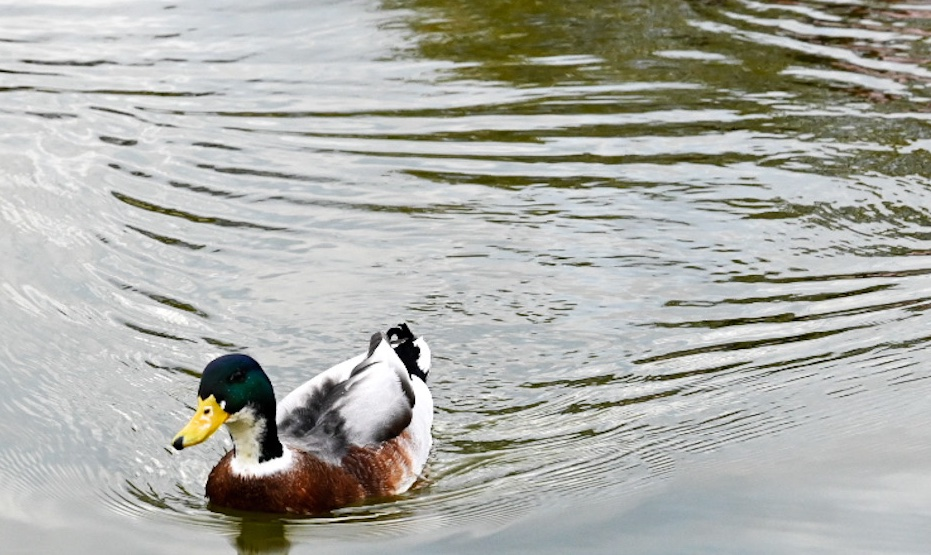
\includegraphics[width=7cm]{duck_wave_pattern.jpg}
    \caption{\textbf{Duck waves.} A duck moving around in a pond produces a wave pattern in its wake (Jardin des Tuileries, Paris. Photograph AA).}
    \label{fig:wave_pattern}
\end{figure}
An object moving at a free surface, such as a boat or an animal, generates a characteristic wave pattern illustrated figure~\ref{fig:wave_pattern}. This pattern is confined in a wedge of half-opening angle $\theta$, remarkably constant across the scales. In the following we set out to determine this angle..
\begin{enumerate}
\item The pulsation $\omega$ of a monochromatic water wave is given by:
\begin{equation}
\omega^2=gk\tanh kh.
\end{equation}
Here $k$, $g$ and $h$ stand respectively for the wavenumber, the gravity and the water depth.
Determine the phase velocity $c$.
\item Express the group velocity $c_g$ as a function of $c$.
\item Find the asymptotic expressions of $c$ and $c_g$ in the deep water limit.
\end{enumerate}
A key assumption in the determination of the wave pattern lies in the fact that the pattern appears \textit{steady} or frozen from the point of view of an observer moving with the boat.
\begin{enumerate}[resume]
\item Find the phase velocity of a steady wavefront moving in the direction of the boat.
\item Steady wavefronts are such that the (prolongated) crests pass through the boat. Find the phase velocity of a steady wavefront whose direction of propagation forms an angle  $\alpha$ with the velocity of the boat. 
\item By considering all possible directions deduce the shape of the wave pattern produced by the boat. 
\item Remembering that wavepackets propagate at the group velocity $c_g$ refine your prediction and obtain the semi-angle characterizing \textit{Kelvin's wedge} enclosing the wave pattern:
\begin{equation}
\theta = \arcsin\lp\tfrac{1}{3}\rp.
\end{equation}
\end{enumerate}

\section{Asymptotic shape of a wavetrain}
The Korteweg-de Vries equation describes the propagation of wave by considering first-order dispersive effects:
\begin{equation}
\frac{\partial\eta}{\partial t}+c_0\frac{\partial \eta}{\partial x}+\frac{c_0 h_0^2}{6}\frac{\partial^3\eta}{\partial x^3}=0.
\end{equation}
In the following we consider a wavepacket generated near the origin at initial time, and we seek to determine the asymptotic shape of the wavetrain far from the origin. We assume that the free surface elevation is a known data and that the wave height decreases to zero at infinity:
\begin{equation}
\int_{-\infty}^{\infty} \eta \, \mathrm dx = A \quad \text{ and } \quad \lim_{x\to\infty} \eta = 0.
\end{equation}
\begin{enumerate}
\item Demonstrate that this equation describes dispersive waves (Hint: insert a wavelike disturbance and compute the phase velocity).
\item Rewrite this equation in a frame moving at velocity $c_0$, i.e. using $\xi = x - c_0t$ and $t$.
\end{enumerate}
In the following, we look for a \textit{scale invariant} solution of the Korteweg-de Vries equation.
\begin{enumerate}[resume]
\item Writing $\alpha = c_0 h_0^2$, find the relations linking the scale factors.
\item Show that $\eta(\xi,t)$ can be represented as:
\begin{equation}
\eta(\xi,t)=\frac{1}{\lp\alpha t\rp^{1/3}}f(\mu),
\end{equation}
where $\mu$ is a similitude variable to be precised.
\item Insert this functional relation into Korteweg-de Vries equation and determine the self-similar shape of the free surface.
\end{enumerate} 
\prg{Airy's function.} The solution to:
\begin{equation}
y''(x)=xy(x)
\end{equation}
is Airy's function Ai($x$). This function satisfies $\lim_{x\to\infty}\mathrm{Ai}(x) = 0$ and $\int_{-\infty}^\infty \mathrm{Ai}(u)\,\mathrm du = 1$.
\begin{figure}[ht]
    \centering
    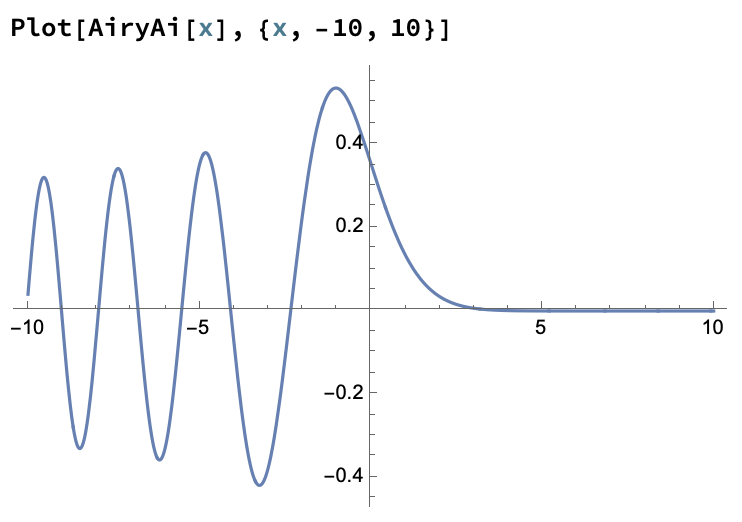
\includegraphics[width=7cm]{airy.png}
    \caption{\textbf{Airy's function.}}
    \label{fig:airy}
\end{figure}
\bibliographystyle{jfm}
\bibliography{biblio_tuto}
\end{document}